%  A simple AAU report template.
%  2015-05-08 v. 1.2.0
%  Copyright 2010-2015 by Jesper Kjær Nielsen <jkn@es.aau.dk>
%
%  This is free software: you can redistribute it and/or modify
%  it under the terms of the GNU General Public License as published by
%  the Free Software Foundation, either version 3 of the License, or
%  (at your option) any later version.
%
%  This is distributed in the hope that it will be useful,
%  but WITHOUT ANY WARRANTY; without even the implied warranty of
%  MERCHANTABILITY or FITNESS FOR A PARTICULAR PURPOSE.  See the
%  GNU General Public License for more details.
%
%  You can find the GNU General Public License at <http://www.gnu.org/licenses/>.
%
\documentclass[11pt,twoside,a4paper,openright]{report}
%%%%%%%%%%%%%%%%%%%%%%%%%%%%%%%%%%%%%%%%%%%%%%%%
% Language, Encoding and Fonts
% http://en.wikibooks.org/wiki/LaTeX/Internationalization
%%%%%%%%%%%%%%%%%%%%%%%%%%%%%%%%%%%%%%%%%%%%%%%%
% Select encoding of your inputs. Depends on
% your operating system and its default input
% encoding. Typically, you should use
%   Linux  : utf8 (most modern Linux distributions)
%            latin1 
%   Windows: ansinew
%            latin1 (works in most cases)
%   Mac    : applemac
% Notice that you can manually change the input
% encoding of your files by selecting "save as"
% an select the desired input encoding. 
\usepackage[utf8]{inputenc}
% Make latex understand and use the typographic
% rules of the language used in the document.
\usepackage[danish]{babel}
% Use the palatino font
\usepackage[sc]{mathpazo}
\linespread{1.05}         % Palatino needs more leading (space between lines)
% Choose the font encoding
\usepackage[T1]{fontenc}
%%%%%%%%%%%%%%%%%%%%%%%%%%%%%%%%%%%%%%%%%%%%%%%%
% Graphics and Tables
% http://en.wikibooks.org/wiki/LaTeX/Importing_Graphics
% http://en.wikibooks.org/wiki/LaTeX/Tables
% http://en.wikibooks.org/wiki/LaTeX/Colors
%%%%%%%%%%%%%%%%%%%%%%%%%%%%%%%%%%%%%%%%%%%%%%%%
% load a colour package
\usepackage{xcolor}
\definecolor{aaublue}{RGB}{33,26,82}% dark blue
% The standard graphics inclusion package
\usepackage{graphicx}
\graphicspath{{./graphics/}}
% Set up how figure and table captions are displayed
\usepackage{caption}
\captionsetup{%
  font=footnotesize,% set font size to footnotesize
  labelfont=bf % bold label (e.g., Figure 3.2) font
}
\usepackage{pdfpages}
\usepackage[numbers, sort&compress]{natbib}
% Make the standard latex tables look so much better
\usepackage{array,booktabs}
% Enable the use of frames around, e.g., theorems
% The framed package is used in the example environment
\usepackage{framed}
\usepackage[linewidth=2pt]{mdframed} %Bliver brugt til at lave en ramme om ting

%%%%%%%%%%%%%%%%%%%%%%%%%%%%%%%%%%%%%%%%%%%%%%%%
% Mathematics
% http://en.wikibooks.org/wiki/LaTeX/Mathematics
%%%%%%%%%%%%%%%%%%%%%%%%%%%%%%%%%%%%%%%%%%%%%%%%
% Defines new environments such as equation,
% align and split 
\usepackage{amsmath}
% Adds new math symbols
\usepackage{amssymb}
% Use theorems in your document
% The ntheorem package is also used for the example environment
% When using thmmarks, amsmath must be an option as well. Otherwise \eqref doesn't work anymore.
\usepackage[framed,amsmath,thmmarks]{ntheorem}

%%%%%%%%%%%%%%%%%%%%%%%%%%%%%%%%%%%%%%%%%%%%%%%%
% Page Layout
% http://en.wikibooks.org/wiki/LaTeX/Page_Layout
%%%%%%%%%%%%%%%%%%%%%%%%%%%%%%%%%%%%%%%%%%%%%%%%
% Change margins, papersize, etc of the document
\usepackage[
  inner=28mm,% left margin on an odd page
  outer=41mm,% right margin on an odd page
  ]{geometry}
% Modify how \chapter, \section, etc. look
% The titlesec package is very configureable
\usepackage{titlesec}
\titleformat{\chapter}[display]{\normalfont\huge\bfseries}{\chaptertitlename\ \thechapter}{20pt}{\Huge}
\titleformat*{\section}{\normalfont\Large\bfseries}
\titleformat*{\subsection}{\normalfont\large\bfseries}
\titleformat*{\subsubsection}{\normalfont\normalsize\bfseries}
%\titleformat*{\paragraph}{\normalfont\normalsize\bfseries}
%\titleformat*{\subparagraph}{\normalfont\normalsize\bfseries}

% Clear empty pages between chapters
\let\origdoublepage\cleardoublepage
\newcommand{\clearemptydoublepage}{%
  \clearpage
  {\pagestyle{empty}\origdoublepage}%
}
\let\cleardoublepage\clearemptydoublepage

% Change the headers and footers
\usepackage{fancyhdr}
\pagestyle{fancy}
\fancyhf{} %delete everything
\renewcommand{\headrulewidth}{0pt} %remove the horizontal line in the header
\fancyhead[RE]{\small\nouppercase\leftmark} %even page - chapter title
\fancyhead[LO]{\small\nouppercase\rightmark} %uneven page - section title
\fancyhead[LE,RO]{\thepage} %page number on all pages
% Do not stretch the content of a page. Instead,
% insert white space at the bottom of the page
\raggedbottom
% Enable arithmetics with length. Useful when
% typesetting the layout.
\usepackage{calc}

%%%%%%%%%%%%%%%%%%%%%%%%%%%%%%%%%%%%%%%%%%%%%%%%
% Bibliography
% http://en.wikibooks.org/wiki/LaTeX/Bibliography_Management
%%%%%%%%%%%%%%%%%%%%%%%%%%%%%%%%%%%%%%%%%%%%%%%%
%\usepackage[backend=bibtex,
%  bibencoding=utf8
%  ]{biblatex}
%\addbibresource{bib}

%%%%%%%%%%%%%%%%%%%%%%%%%%%%%%%%%%%%%%%%%%%%%%%%
% Misc
%%%%%%%%%%%%%%%%%%%%%%%%%%%%%%%%%%%%%%%%%%%%%%%%
% Add bibliography and index to the table of
% contents
\usepackage[nottoc]{tocbibind}
% Add the command \pageref{LastPage} which refers to the
% page number of the last page
\usepackage{lastpage}
% Add todo notes in the margin of the document
\usepackage[
%  disable, %turn off todonotes
  colorinlistoftodos, %enable a coloured square in the list of todos
  textwidth=\marginparwidth, %set the width of the todonotes
  textsize=scriptsize, %size of the text in the todonotes
  ]{todonotes}

%%%%%%%%%%%%%%%%%%%%%%%%%%%%%%%%%%%%%%%%%%%%%%%%
% Hyperlinks
% http://en.wikibooks.org/wiki/LaTeX/Hyperlinks
%%%%%%%%%%%%%%%%%%%%%%%%%%%%%%%%%%%%%%%%%%%%%%%%
% Enable hyperlinks and insert info into the pdf
% file. Hypperref should be loaded as one of the 
% last packages
\usepackage{hyperref}
\hypersetup{%
	pdfpagelabels=true,%
	plainpages=false,%
	pdfauthor={Author(s)},%
	pdftitle={Title},%
	pdfsubject={Subject},%
	bookmarksnumbered=true,%
	colorlinks=true,%
	citecolor=black,%
	filecolor=black,%
	linkcolor=black,% you should probably change this to black before printing
	urlcolor=black,%
	pdfstartview=FitH%
}

\usepackage{enumitem}
\usepackage{caption}
\usepackage{subcaption}
\usepackage{cleveref}
\usepackage{listings}

% see, e.g., http://en.wikibooks.org/wiki/LaTeX/Formatting#Hyphenation
% for more information on word hyphenation
\hyphenation{ex-am-ple hy-phen-a-tion short}
\hyphenation{long la-tex}

%  A simple AAU report template.
%  2015-05-08 v. 1.2.0
%  Copyright 2010-2015 by Jesper Kjær Nielsen <jkn@es.aau.dk>
%
%  This is free software: you can redistribute it and/or modify
%  it under the terms of the GNU General Public License as published by
%  the Free Software Foundation, either version 3 of the License, or
%  (at your option) any later version.
%
%  This is distributed in the hope that it will be useful,
%  but WITHOUT ANY WARRANTY; without even the implied warranty of
%  MERCHANTABILITY or FITNESS FOR A PARTICULAR PURPOSE.  See the
%  GNU General Public License for more details.
%
%  You can find the GNU General Public License at <http://www.gnu.org/licenses/>.
%
%
%
% see, e.g., http://en.wikibooks.org/wiki/LaTeX/Customizing_LaTeX#New_commands
% for more information on how to create macros

%%%%%%%%%%%%%%%%%%%%%%%%%%%%%%%%%%%%%%%%%%%%%%%%
% Macros for the titlepage
%%%%%%%%%%%%%%%%%%%%%%%%%%%%%%%%%%%%%%%%%%%%%%%%
%Creates the aau titlepage
\newcommand{\aautitlepage}[3]{%
  {
    %set up various length
    \ifx\titlepageleftcolumnwidth\undefined
      \newlength{\titlepageleftcolumnwidth}
      \newlength{\titlepagerightcolumnwidth}
    \fi
    \setlength{\titlepageleftcolumnwidth}{0.5\textwidth-\tabcolsep}
    \setlength{\titlepagerightcolumnwidth}{\textwidth-2\tabcolsep-\titlepageleftcolumnwidth}
    %create title page
    \thispagestyle{empty}
    \noindent%
    \begin{tabular}{@{}ll@{}}
      \parbox{\titlepageleftcolumnwidth}{
        \iflanguage{danish}{%
          
\includegraphics[width=.8\titlepageleftcolumnwidth]{aau_logo_da}
        }{%
          
\includegraphics[width=.8\titlepageleftcolumnwidth]{aau_logo_en}
        }
      } &
      \parbox{\titlepagerightcolumnwidth}{\raggedleft\sf\small
        #2
      }\bigskip\\
       #1 &
      \parbox[t]{\titlepagerightcolumnwidth}{%
      \textbf{Abstract:}\bigskip\par
        \fbox{\parbox{\titlepagerightcolumnwidth-2\fboxsep-2\fboxrule}{%
          #3
        }}
      }\\
    \end{tabular}
    \vfill
    \iflanguage{danish}{%
      \noindent{\footnotesize\emph{Rapportens indhold er frit tilgængeligt, men offentliggørelse (med kildeangivelse) må kun ske efter aftale med forfatterne.}}
    }{%
      \noindent{\footnotesize\emph{The content of this report is freely available, but publication (with reference) may only be pursued due to agreement with the author.}}
    }
    \clearpage
  }
}

%Create english project info
\newcommand{\englishprojectinfo}[8]{%
  \parbox[t]{\titlepageleftcolumnwidth}{
    \textbf{Title:}\\ #1\bigskip\par
    \textbf{Theme:}\\ #2\bigskip\par
    \textbf{Project Period:}\\ #3\bigskip\par
    \textbf{Project Group:}\\ #4\bigskip\par
    \textbf{Participant(s):}\\ #5\bigskip\par
    \textbf{Supervisor(s):}\\ #6\bigskip\par
    \textbf{Copies:} #7\bigskip\par
    \textbf{Page Numbers:} \pageref{LastPage}\bigskip\par
    \textbf{Date of Completion:}\\ #8
  }
}

%Create danish project info
\newcommand{\danishprojectinfo}[8]{%
  \parbox[t]{\titlepageleftcolumnwidth}{
    \textbf{Titel:}\\ #1\medskip \par
    \textbf{Tema:}\\ #2\medskip \par
    \textbf{Projektperiode:}\\ #3\medskip \par
    \textbf{Projektgruppe:}\\ #4\medskip \par
    \textbf{Deltager(e):}\\ #5\medskip \par
    \textbf{Vejleder(e):}\\ #6\medskip \par
    \textbf{Oplagstal:} #7\medskip \par
    \textbf{Sidetal:} \pageref{LastPage}\medskip \par
    \textbf{Afleveringsdato:}\\ #8
  }
}

%%%%%%%%%%%%%%%%%%%%%%%%%%%%%%%%%%%%%%%%%%%%%%%%
% An example environment
%%%%%%%%%%%%%%%%%%%%%%%%%%%%%%%%%%%%%%%%%%%%%%%%
\theoremheaderfont{\normalfont\bfseries}
\theorembodyfont{\normalfont}
\theoremstyle{break}
\def\theoremframecommand{{\color{gray!50}\vrule width 5pt \hspace{5pt}}}
\newshadedtheorem{exa}{Example}[chapter]
\newenvironment{example}[1]{%
		\begin{exa}[#1]
}{%
		\end{exa}
}

\newcommand{\namedtodo}[5]
{
  \ifthenelse{\equal{#1}{}}
  {
    \todo[backgroundcolor=#4,linecolor=#4,caption=
    {\textbf{#3: } #2}]
    {\color{#5}\textbf{#3: }#2}
  }
  {
    \todo[backgroundcolor=#4,linecolor=#4,caption=
    {\textbf{#3: } #1}]
    {\color{#5}\textbf{#3: }#2}
  }
}
\newcommand{\namedtodoinline}[5]
{
  \ifthenelse{\equal{#1}{}}
  {
    \todo[backgroundcolor=#4,caption=
    {\textbf{#3: } #2}
    ,inline]
    {\normalsize\color{#5}\textbf{#3: }#2}
  }
  {
    \todo[backgroundcolor=#4,caption=
    {\textbf{#3: } #1}
    ,inline]
    {\normalsize\color{#5}\textbf{#3: }#2}
  }
}
\newcommand{\mikkel}[2][]{\namedtodo{#1}{#2}{Mikkel}{blue!80}{white}}
\newcommand{\mikkelin}[2][]{\namedtodoinline{#1}{#2}{Mikkel}{blue!80}{white}}
\newcommand{\stefan}[2][]{\namedtodoinline{#1}{#2}{Stefan M}{orange}{black}}
\newcommand{\mikael}[2][]{\namedtodoinline{#1}{#2}{Mikael}{green}{black}}
\newcommand{\bruno}[2][]{\namedtodoinline{#1}{#2}{Bruno}{black!10!red!90}{white}}

\makeatletter \renewcommand \listoftodos{\section*{List of Todos} \@starttoc{tdo}}
\renewcommand\l@todo[2]
  {\par\noindent \textit{#2}, \parbox{10cm}{#1}\par} \makeatother
% Her er en liste over navnene på de forskellige styles
% C#: csharp
% F#: fsharp

% 
% Listings kan refereres vha. \cref{}
\crefname{lstlisting}{kode eksempel}{kode eksempler}
\Crefname{lstlisting}{Kode eksempel}{Kode eksempler}
\renewcommand{\lstlistingname}{Kode eksempel}
\renewcommand{\lstlistlistingname}{Liste af kode eksempler}
%

%Algoritmer i cref
\crefname{algocf}{algoritmne}{algoritmne}
\Crefname{algocf}{Algoritmne}{Algoritmne}
%Algoritmelinjer i cref
\crefalias{AlgoLine}{line}%

\makeatletter
\let\cref@old@stepcounter\stepcounter
\def\stepcounter#1{%
  \cref@old@stepcounter{#1}%
  \cref@constructprefix{#1}{\cref@result}%
  \@ifundefined{cref@#1@alias}%
    {\def\@tempa{#1}}%
    {\def\@tempa{\csname cref@#1@alias\endcsname}}%
  \protected@edef\cref@currentlabel{%
    [\@tempa][\arabic{#1}][\cref@result]%
    \csname p@#1\endcsname\csname the#1\endcsname}}
\makeatother
%

\lstdefinestyle{standard}
{
	frame=shadowbox,
	framesep=5pt,
	rulecolor=\color{blue!40!black},
	rulesepcolor=\color{white!93!black},
	numbers=left,
	basicstyle=\ttfamily,
	numberstyle=\tiny,
	numberfirstline=true,
	%numberblanklines=false,
	stepnumber=1,
	numbersep=9pt,	
	captionpos=b,
	escapeinside={(*}{*)},
	breaklines=true,
	tabsize=4,
	language=c,
	showstringspaces=false
}

\lstset{style=standard}

\lstdefinestyle{c}
{
	style=standard
}

\lstdefinestyle{csmall}
{
	style=c
}

\lstdefinestyle{csharp}
{
	style=standard,
	language=[Sharp]C
}
\lstdefinestyle{csharpsmall}
{
	style=csharp
}
\lstdefinestyle{fsharp}
{
	language=[Sharp]F,
	frame=lr,
	rulecolor=\color{blue!80!black}
}
\lstdefinestyle{fsharpsmall}
{
	style=fsharp,
	basicstyle=\ttfamily\footnotesize
}


% Definitions
\newcommand{\projectname}{PsyLog2\xspace}

% Superscript and subscript
\newcommand{\superscript}[1]{\ensuremath{^{\textrm{#1}}}}
\newcommand{\subscript}[1]{\ensuremath{_{\textrm{#1}}}}

% Degrees
\newcommand{\degree}{\ensuremath{^\circ}}
\newcommand{\dg}{\degree}

\newcommand{\quoter}[1]%
{
  \par
  \vspace{1.5em}
  \addtolength{\leftskip}{1.5cm}
  \addtolength{\rightskip}{1.5cm}
  \textit{#1}
  \addtolength{\leftskip}{-1.5cm}
  \addtolength{\rightskip}{-1.5cm}
  \vspace{1.5em}
  \par
}


\begin{document}

%Front page
\begin{titlepage}

\begin{center}
\newcommand{\HRule}{\rule{\linewidth}{0.5mm}}
\HRule \\[0.4cm]
\textsc{ \Huge Affektive Lidelser: Forstyrrende og Ikke-Forstyrrende Indsamling af Data om Social Aktivitet \\[0.3cm]
	\Large Del af PsyLog }\\[0.4cm]

\HRule \\[1cm]

\textsc{\Large SW807F15} \\[2cm]


\includegraphics[width=.5\textwidth]{logo}

\vfill
{\Large Mobilteknologi}
\\ ~\\
{\large 8. Semester, Foråret 2015}

\end{center}
\end{titlepage}

\setcounter{secnumdepth}{3}

\cleardoublepage

\pdfbookmark[0]{Titelblad}{label:titlepage_da}
\aautitlepage{%
  \danishprojectinfo{
    %title
    PsyLog - En modulær mobil platform
  }{%
    Mobile Systemer %theme
  }{%
    Forårssemestret 2015 %project period
  }{%
    SW807 % project group
  }{%
    %list of group members
    Bruno Thalmann\\
    Mikael Elkiær Christensen\\
    Mikkel Larsen\\
    Stefan Marstrand Getreuer Micheelsen
  }{%
    %list of supervisors
    Ivan Aaen
  }{%
    1 % number of printed copies
  }{%
    \today % date of completion
  }%
}{%department and address
  \textbf{Information og kommunikations teknologi}\\
  Selma Lagerlöfsvej 300\\
  Aalborg Universitet\\
  \href{http://www.aau.dk}{http://www.aau.dk}
}{% the abstract
  \stefan{abstract}
}


\cleardoublepage

\pagenumbering{Roman}
\setcounter{page}{1}
\newcommand{\prefaceHeaderName}{Preface}
\section*{\prefaceHeaderName}
This report has been prepared by 7th semester Software Engineering students at Aalborg University, during the fall-semester of 2014.
It is expected of the reader to have a background in IT/software, due to the technical content.

References and citations are done by the use of numeric notation, e.g. \cite{civitas-archimedes}, which refers to the first item in the bibliography.

In the report, this project will henceforth be referred to as \projectname.
Whenever the report refers to 'we', it is to be understood as the members of the project group sw701e14.

Finally, we would like to thank our lecturers, and an especially big thanks to our supervisor Giovanni Bacci, for his excellent supervision throughout the semester.


%Table of contents
\pdfbookmark{\contentsname}{toc}
\setcounter{tocdepth}{1}
\tableofcontents

\cleardoublepage

\pagenumbering{arabic}

\newcommand{\introductionHeaderName}{Introduktion}
\chapter*{\introductionHeaderName}
\addcontentsline{toc}{chapter}{\introductionHeaderName}
Dette projekt bygger videre på det fundament som blev udarbejdet i \cref{}\footnote{Fællesrapporten}.

Som det kan ses ud fra \cref{?}\footnote{Fællesrapport, Kapitel 'Indsamling af data'} er der mange muligheder for indsamling og logning af data via mobile enheder.
De faktorer som vurderes de vigtigste og mest effektive, baseret på de to person interviews, samt fokusgruppeinterviewet, er søvn og social aktivitet.
Den anden af de to grupper har valgt at fokusere på søvn, hvorfor dette projekt vil fokusere på det sociale.

Gennem interviewet med Jørgen Aagaard, blev det slået fast at det sociale spiller en væsentlig rolle ved detektering af episoder.
Ved depression mindskes det hvor meget der siges og skrives og aktiviteter vil blive nedsat.
Ved mani vil det være modsat, da der vil være en stigning i kontakt udadtil.
Det er derved interessant at måle og observere ændringer i mængden af social kontakt.

For at være i stand til at kunne måle på disse ændringer, skal der fastslås en model og derudfra en baseline.
Herefter bliver det bliver muligt at sammenligne målt adfærd med tidligere adfærd, og derved observere ændringer.

\section{Dataindsamling}
I \cref{?}\footnote{Fællesrapport, Sektion 3.3 Mobil logning} blev der nævnt adskillige muligheder for logning på mobiltelefon.
Disse var; opkald, applikationsbrug og SMS/MMS.
Derudover blev der i \cref{?}\footnote{Fællesrapport, Sektion 3.1 Sensorer} nævnt GPS, hvilket også ville kunne blive brugt som indikation på aktivitet, herunder social aktivitet.

Eksempler på brugen af disse logninger, i forbindelse med symptomerne (se \cref{?}\footnote{Fællesrapporten, Sektion 1.21 Depression og 1.2.2 Mani}), blev analyseret i \cref{?}\footnote{Fællesrapporten, Sektion 3.4}.
Disse vil blive uddybet her, med fordele og begrænsninger ved de forskellige logninger.

Ved relatering til patienters adfærd, antages det at disse er udenfor, eller mellem, episode.
Derved antages det at disse fungerer som almindelige mennesker, der går på arbejde eller i skole og deltager i andre aktiviteter (herunder sociale).

\subsection{GPS}
Via smartphone, eller wearable som understøtter dette, er det muligt at forespørge på brugerens nuværende lokation.
Dette resulterer, som minimum, i en længdegrad, breddegrad og præcision.
Derudover kan flere forespørgsler kombineres til at sige noget om retning, hastighed og acceleration.

Nogle patienter vil de deltage i sociale aktiviteter, såsom sport eller anden klub-aktivitet, fest og generel social aktivitet med familie eller venner.
Så ville man over tid kunne identificere disse lokationer, da de ville være tilbagevendende.
Evt. kunne man få bruger-input til præcist at identificere nogle af disse lokationer.
Når først disse lokationer er bestemt, vil man kunne danne en model over den enkelte patients aktivitets-mønster.

Ved at skelne mellem sociale og ikke-sociale lokationer (ens hjem, muligvis andre), ville man kunne registrere ændringer i den sociale aktivitet.
Ud fra den viden der er dannet i fællesrapporten, vil der for patienter på vej ind i en depression være et fald i social aktivitet.
For patienter på vej ind i en mani vil der omvendt være en stigning.

\paragraph{Begrænsninger}
Ved GPS-lokation alene, er det ikke direkte muligt at sige om en aktivitet er social eller ikke.
Der vil være situationer hvor man er i ens hjem en hel weekend, men muligvis har besøg af venner eller familie.
Omvendt kunne man også tage til en familiebegivenhed, hvor man ikke nødvendigvis snakker eller på anden måde socialiserer med nogen.

\section{Opkald}
På Android-smartphones er det muligt at få adgang til opkalds-historikken.
Her kan man se indgående, udgående og missede opkald, samt modtager/afsender og varighed.

Opkalds-historikken alene kan give et billede af kvantiteten for opkald, samt en smule om kvaliteten via opkaldets varighed.
Ved at tælle antallet af opkald, ville man kunne observere en ændring ved henholdsvis begyndende depression eller mani.
Ved depression antages det at antallet af opkald, især udgående, vil falde.
Det antages også at længden af opkaldene vil være kortere end normalt.
Som benævnt i fokusgruppe-interviewet, vil ens netværk også mindskes, hvilket vil kunne ses på modtager/afsender på opkaldene, hvor antal forskellige kontaktpersoner vil falde.
Derimod vil man ved mani forvente en stigning i opkald, især udgående.
Der vil også være en stigning i antal forskellgie udgående kontakter.

\paragraph{Begrænsninger}
Da der kun ses på opkalds-historikken, er det ikke muligt at sige noget om kvaliteten af opkaldene.
Det vil sige at der ikke kan siges noget om hvor meget der bliver sagt af patienten, eller af afsender/modtager.

For mange personer vil der være begrænset brug af telefon-opkald, da der også vil foregå en stor del af den samme slags kommunikation via Facebook, Whatsapp, Skype eller lignende.

\section{SMS/MMS beskeder}
Ligesom opkalds-historik, er der indbygget i Android mulighed for adgang til SMS/MMS-historik.
Her kan man få en liste over beskeder, med for hver besked afsender/modtager, indhold (og derudaf længden), afsendt/modtaget tidspunkt og om hvorvidt det er en sendt eller modtaget besked.

Observation af beskeder vil fungere i høj grad på samme måde som opkald.

\paragraph{Begrænsninger}
For mange personer vil der være begrænset brug af SMS/MMS-beskeder, da der også vil foregå en stor del af den samme slags kommunikation via Facebook, Whatsapp, Skype eller lignende.

\section{Applikations-brug}
I nyere versioner af Android er det muligt at få adgang til brugs-statistik for alle installerede applikationer.
Her er det muligt at forespørge på forskellige tidsintervaller, hvilket resulterer i en liste af applikationer brugt i tidsintervallet.
For hver applikation vil der være informationer omkring totalt tidsforbrug i millisekunder, tidligste og seneste brug (indenfor tidligere angivet interval).

Med denne information er det muligt at se hvor meget tid der bruges på applikationer med socialt indhold, som for eksempel Facebook, Skype e.l.

\paragraph{Begrænsninger}
Dette er kun muligt for nyere versioner af Android; fra og med API version 21, eller Androd 5.0 Lollipop.
Det vil heller ikke være muligt at se hvad de forskellige apps har været brugt til, men kun i hvor lang tid.
For eksempel vil man for Facebook-app'en ikke kunne se om der er brugt tid på at skrive til andre, læse nyheder eller spillet spil.


\chapter{Begreber}
For at opnå en fælles forståelse for både psykologiske begreber samt begreber introduceret af projektgruppen samles her definitioner af de vigtigste begreber der bruges i rapporten.

\section[Affektive fænomener]{Affektive fænomener \footnote{Engelsk: affective phenomena}}
Dette afsnit introducerer de tre fænomener affekt, følelse og humør, hvor fællesbetegnelsen benævnes \textit{affektive fænomener}.
Denne introduktion, samt de efterfølgende definitioner, er baseret på oversættelser af \citet{ekkekakis}.

Affektive fænomener er et stort og komplekst område.
De tre førnævnte begreber er nært relateret, hvilket har resulteret i adskillige teorier.
Der er stor uenighed indenfor psykologien hvad de tre begreber hver især dækker over, samt hvordan de hænger sammen.
I \citet{ekkekakis} siges det at det ikke er muligt at skabe en dyb nok forståelse for dette uden at læse et væld af artikler, til gengæld gives denne korte introduktion (de følgende definitioner af fænomenerne) hvorefter det opfordres at kigge på de angivne kilder, samt foretage egen undersøgelse.
De præsenterede definitioner er vores opfattelse af begreberne, og disse betydninger vil blive benyttet igennem rapporten.


\subsection[Affekt]{Affekt\footnote{Engelsk: affect}}
Affekt beskriver en neurologisk tilstand, som er bevidst tilgængelig.
Den er en simpel, ikke-refleksiv fornemmelse, som oftest kommer til syne gennem følelse og humør, men er altid til stede for bevidstheden.

Eksempler på affekt inkluderer glæde og sorg, afslappethed og anspændthed, energi og træthed.
Affekt kan være en isoleret, ren fornemmelse, men kan også indgå i en følelse eller et humør.

Et mere konkret eksempel er \textit{stolthed}, hvor man har det godt med sig selv.
Det at \textit{have det godt} er affekt, og \textit{med sig selv} er noget kognitivt.
Dette kvalificerer \textit{stolthed} som en følelse.\cite[p. 322]{ekkekakis}

\subsection[Følelse]{Følelse\footnote{Engelsk: feeling}}
En typisk følelsesmæssig episode kan beskrives som en kompleks mængde af sammenhængende omstændigheder vedrørende et specifikt objekt, hvor dette objekt kan være en person, begivenhed eller genstand, uafhængigt af tid og virkelighed.

De sammenhængende omstændigheder dækker over a) affekt, b) synlig opførsel knyttet til følelsen (e.g. smil eller vidt-åbne øjne), c) opmærksomhed rettet mod katalysatoren, d) kognitiv vurdering af betydning og konsekvenser af katalysatoren, e) tillæggelse af begivenhederne der startede katalysatoren, f) oplevelsen af den pågældende følelse, g) neurale og endokrine ændringer som resultat af den pågældende følelse.

Eksempler på følelser er vrede, frygt, jalousi, stolthed og kærlighed.\cite[p. 322]{ekkekakis}

\subsection[Humør]{Humør\footnote{Engelsk: mood}}
Noget som gør at humør skiller sig ud fra affekt og følelse, er at de typisk er længere-varende.
Humør er også ofte beskrevet som noget mere diffust og globalt, modsat specifikt.
Humør er den passende betegnelse for affektive tilstande der omhandler intet specifikt, eller alt -- generelt om verden.

Eksempelvis kan for en person som er bekymret (som er et humør), et objekt være fremtiden.
Ved en deprimeret person kunne objektet være personen selv som helhed.
For en irriteret person kan objektet være hvem eller hvad som helst.

Til forskel fra følelse, er katalysatoren for humør noget tidsmæssigt fjernt (e.g. en person kan vågne i dårligt humør som resultat af en hændelse den forrige dag).
Dette resulterer i at det ikke altid er klart hvordan et humør er opstået.\cite[p. 322]{ekkekakis}

\paragraph{Stemningsleje} er et andet begreb ofte brugt i forbindelse med affektive lidelser.
Umiddelbart dækker det over det samme som humør, da det beskriver noget længerevarende.
På samme måde som man kan være i godt eller dårligt humør, kan man have hævet eller sænket stemningsleje.

\section{Forstyrrende og ikke-forstyrrende dataindsamling}
Som det kan ses i titlen på rapporten, skelnes der overordnet mellem to typer af dataindsamling; forstyrrende og ikke-forstyrrende.

\subsection{Forstyrrende dataindsamling}\label{begreber::forstyrrende}
Med forstyrrende menes der at der aktivt skal foretages noget af brugeren for at der kan leveres data om brugeren.
Det menes ikke som noget direkte negativt, blot at det er mere forstyrrende i forhold til dataindsamling som kan foregå i baggrunden uden bruger-interaktion.
Eksempler på forstyrrende dataindsamling kunne være at tage et billede af sig selv en gang i timen eller at svare på spørgsmål vedrørende sit stemningsleje.

Fordelen ved forstyrrende dataindsamling er at det er nemmere at få adgang til informationer om brugeren, og dennes tilstand, som man ikke umiddelbart kan via sensorer eller anden baggrunds dataindsamling.
Dette kunne være angående brugerens humør eller i hvor høj grad brugeren er sulten.
Ulempen ved denne type data er at den ofte er meget subjektiv. 
Ved at spørge patienten skal brugeren selv tage stilling til sin tilstand og det er derfor muligt for patienten at manipulere med svaret, både bevidst og ubevidst.
Til gengæld kan der indsamles mere objektivt meta-data omkring brugerens besvarelser/interaktioner; såsom besvarelses-tid, antal skift af valg eller annullering.

\subsection{Ikke-forstyrrende dataindsamling}\label{begreber::ikke_forstyrrende}
Modsat den aktive dataindsamling, kræver den ikke-forstyrrende ingen interaktion med brugeren.
Dette gør at brugeren i mindre grad er påvirket af systemet, eller omvendt, og derfor vil den indsamlede data være mindre subjektiv.
Eksempler på ikke-forstyrrende dataindsamling kunne være bevægelsesmønstre via GPS eller optælling af SMS'er og opkald.

Som sagt vil den ikke-forstyrrende indsamlede data oftest være mere objektiv end den forstyrrende indsamlede data.
Dette gør at denne type data vil give et mere realistisk billede af en persons adfærd og stemningsleje.
Dette ligger tæt op ad målet for dette projekt, hvis det er muligt at give et objektivt og præcist billede af stemningsleje uden at dette kan manipuleres af brugeren.

\section{Social aktivitet}
Social aktivitet kan forstås som mange ting.
For de fleste vil det umiddelbart være en fysisk aktivitet foretaget sammen med andre, eller som minimum en aktivitet med en fysisk tilstedeværelse blandt andre.

Ift. dette projekt ses social aktivitet som værende al aktivitet der involverer interaktion med andre personer.
Dette dækker over det fysiske samvær som nævnt ovenover, men også, og måske mere relevant, den interaktion der foregår med andre personer over digitale medier.

Eksempler på sociale aktiviteter, foretaget på smartphone, kunne være den traditionelle brug af en mobiltelefon; opkald og SMS.
Andre eksempler kunne være sociale medier som Facebook eller Twitter.
Det kunne også være multiplayer-spil som 'Wordfeud' eller 'Draw Something'.

\paragraph{Måling af social aktivitet på smartphone} kan foregå på et væld af måder.
Der kan måles både kvantitativt og kvalitativt.

Kvantitativt kan der ses på antal unikke sociale interaktioner i løbet af en dag.
Der kunne også ses på hvor lange disse interaktioner er.

Kvalitativt kunne der ses på hvilken slags aktiviteter der foretages.
Lidt sværere er det at få information om hvordan brugeren har oplevet aktiviteten; om den var behagelig/ubehagelig.

% % % OVERORDNET
% Begreb
% Metode
% Metrik
% Hypotese

% % % ARTIKEL (Mood -> Sociability)
% Hypotese: Positivt humør fører til sociale aktiviteter
% Tidligere: sociale aktiviteter -> affekt
% Metode: Inducering af humør, vurdering af humør, vurdering af fundne aktiviteter

\section{Relevant Forskning}
For at kunne konstruere en model til at repræsentere sammenhængen mellem social aktivitet og sindstilstand, er det nødvendigt først at fastslå en umiddelbar sammenhæng.
Dette gøres ved at undersøge eksisterende forskning indenfor området, som primært er indenfor psykologi-faget.

Vores mål er at mere præcist fastslå denne sammenhæng via mobil data-indsamling.
Dette går imod den måde hvorpå data typisk indsamles indenfor psykologi, hvorfor vi efterfølgende vil undersøge om der allerede er forskning mere relateret til datalogi, hvor denne indsamling foregår mobilt.

\subsection{Sammenhæng mellem humør og social aktivitet}
Ud fra de definitioner der er givet i forrige afsnit, er det humør som vi er interesseret i, da det dækker over længerevarende ændringer, hvilket er tilfældet ved mani-depressive perioder.

For at undersøge den psykologiske forskning og eksperimentering der er foregået op til nu, i forhold til sammenhæng mellem humør og social aktivitet, tages der udgangspunkt i \citet{whelan}.

I denne artikel fastslås det at der er meget forskning der dokumenterer en 2-vejs forbindelse mellem affekt og social aktivitet\footnote{Engelsk: \textit{sociability}}.
Dog har der været begrænset med eksperimentering til at fastslå at godt humør eller positiv affekt fører til mere social aktivitet.
Ud fra en undersøgelse af lignende artikler i den eksisterende forskning, her tages fat i artikler fra 1986 til selve artiklens publikation (2012), kritiseres den relaterede forskning.
De kritiserer nogle af disse tidligere artikler for at komme frem med en tvetydig retning, altså at det ikke er til at vide om humør påvirker social aktivitet eller omvendt.
Derudover er der også kritik til de tidligere brugte metoder, som fejler i at skelne mellem behagelige og sociale aktiviteter.




\subsection{Brug af mobil data-indsamling}
Der er fundet to eksempler på brugen af mobil data-indsamling til at fastslå humør-ændringer; \citet{social_sensing} og \citet{social_sensing_2}.


\section{Survey som Dataindsamling}
For at kunne udlede en sammenhæng mellem stemningsleje og social aktivitet skal der udover målinger af den sociale aktivitet også bruges subjektiv data fra patienten.
Til dette formål skal der konstrueres et modul der kan stille spørgsmål til patienten på varierende tidspunkter.

\subsection{Spørgsmål}\label{survey:spg}
Da der er forskellige metoder til at konsultere en patient om sit stemningsleje er det nødvendigt at kunne stille spørgsmål på forskellige måder.
Der er udvalgt tre typer spørgsmål som vi mener dækker de behov der i forhold til at udspørge patienten både om sin sociale færden og om sit stemningsleje.
Disse typer vil i det følgende blive gennemgået med eksempler på hvilke relevante metoder fra psykologien de kan bruges til.

\paragraph{Multiple choice}
Stemningsregistrering, \cref{stemningsleje::stemningsregistrering}, bruger en skala fra ``svær depression'' til ``svær mani'' til at holde øje med hvor patientens stemningsleje.
Det skal både være muligt at lave spørgsmål hvor man kun kan vælge en mulighed og spørgsmål hvor man kan vælge flere svarmuligheder.
Jævnfør stemningregistrering skalaen skal der kunne tilknyttes en farve til de forkellige muligheder.

\stefan{Hamilton}

\paragraph{Tekst}
For at give mulighed for at patienten kan skrive dagbog \stefan{ref til Måling af stemningsleje} skal der bruges en spørgsmålstype der kan vise en kort tekst som besvares med en tekst fra et tekstfelt.
På denne måde kan der både skrives regulær dagbog, og der kan stilles konkrete spørgsmål såsom ``Hvordan har du ageret socialt i dag?''.

\paragraph{Skala}
I metoden PANAS \stefan{ref til Måling af stemningsleje}stilles patienten et spørgsmål om i hvor høj grad han har følt en bestemt følelse i en vis tidsperiode.
Dette besvares så på en skala fra et til fem.

Vi har altså behov for et spørgsmål der kan besvares med en numerisk skala med mulighed for at sætte labels på skalaen.

\paragraph{Implementation}
De tre typer af spørgsmål er blevet implementeret som kan ses på \cref{sporgsmål}.
På \cref{multi} kan ses en multiple choice spørgsmål hvor der kan vælges flere svarmuligheder.
Dette spørgsmål findes også i en variant hvor man kun kan vælge en mulighed, indikeret ved runde svarbokse (radio buttons).

\Cref{skala} viser et spørgsmål der besvares ved en skala. 
Her vises den med to labels ved minimum og maksimum værdierne.

\Cref{tekst} viser et spørgsmål der skal besvares ved en tekst. 


\begin{figure}
	\centering
	\begin{subfigure}[b]{0.3\textwidth}
		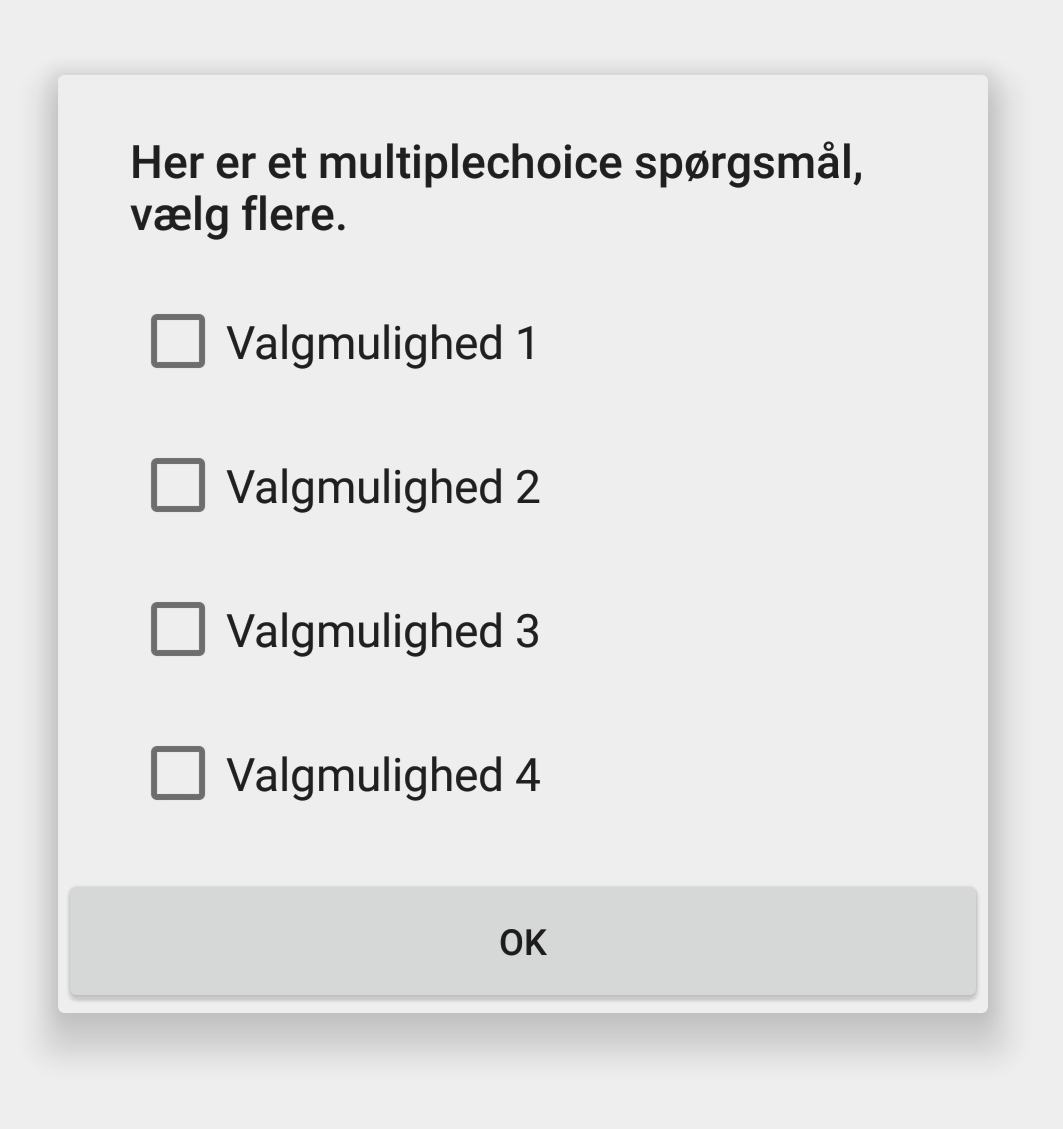
\includegraphics[width=\textwidth]{multiple_choice}
		\caption{Multiple choice}\label{multi}
	\end{subfigure}
	~
	\begin{subfigure}[b]{0.3\textwidth}
		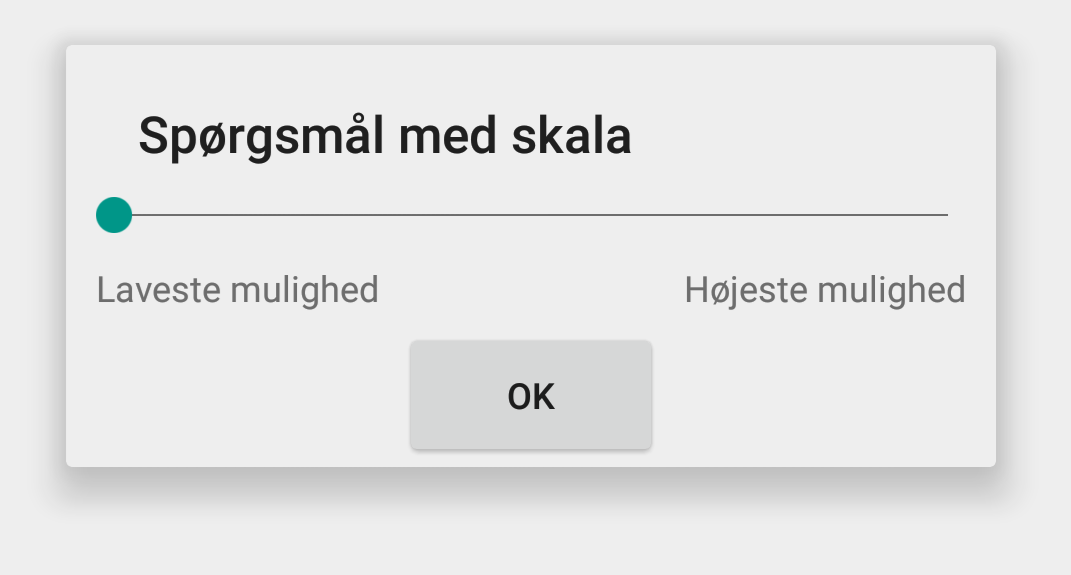
\includegraphics[width=\textwidth]{skala}
		\caption{Skala}\label{skala}
	\end{subfigure}
	~
	\begin{subfigure}[b]{0.3\textwidth}
		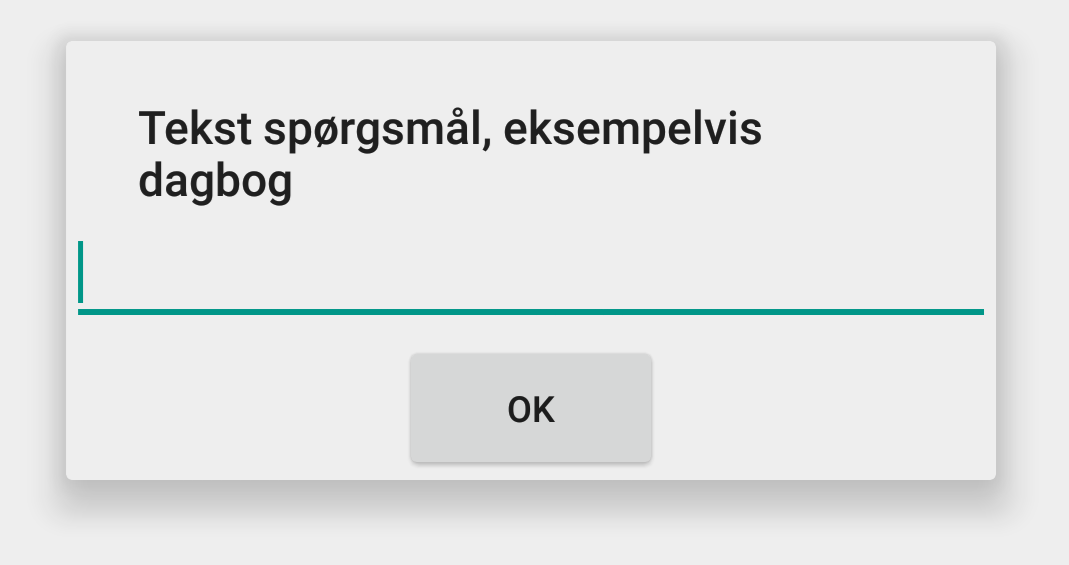
\includegraphics[width=\textwidth]{tekst}
		\caption{Tekst}\label{tekst}
	\end{subfigure}
	\caption{De tre spørgsmålstyper}\label{sporgsmål}
	\stefan{fix afstanden til bunden af billederne}
\end{figure}

\subsection{Scheduler}
For at kunne stille spørgsmål så fleksibelt som muligt er der blevet konstrueret en scheduler.
Stemningsregistrering og dagbog skal ske én gang om dagen, mens PANAS spørgsmål sagtens kan spredes ud over dagen for at få et bredere billede af patientens tilstand.


\paragraph{Notifikationer}
For ikke at forstyrre brugerens hverdag for meget bruger vi en notifikation til at advisere om et forestående spørgsmål.
Notifikationen indeholder spørgsmålsteksten, så patienten kan vurdere om han har tid til at besvare spørgsmålet.
Eksempler på disse notifikationer kan ses på \cref{noti}.

\begin{figure}
	\centering
	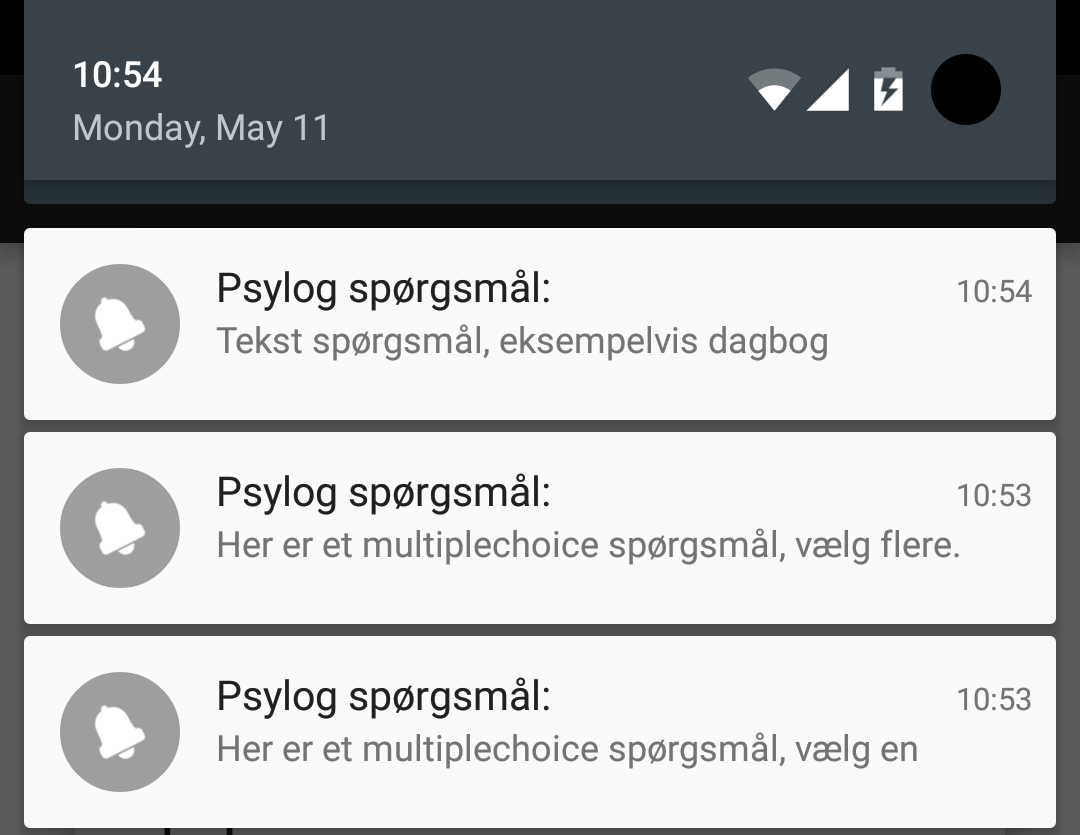
\includegraphics[width=0.6\textwidth]{notifikation}
	\caption{Tre notifikationer sendt af Survey}\label{noti}
\end{figure}

Når der trykkes på notifikationen dukker spørgsmålet op i en dialogboks hvor patientes svar kan indføres.

For at gøre systemet endnu mere fleksibelt skal der være mulighed for at kunne udskyde et spørgsmål.
På denne måde har patienten fuld kontrol over hvornår han svarer, uden at være nødt til at skulle afbryde det han er i gang med.
Dette er endnu ikke implementeret.

\chapter{Beskrivelse af Løsning}

\chapter{Konklusion}

\chapter{Refleksion}
%Til survey: Tilføj "huskekort" - som får patienten til at vykel en tur, yoga etc. - enten at appen selv finder ud af det eller at det er spykologen der løbende kan lægge dem ind.
\label{refleksion}

\bruno{Split måske i diskussio  og refleksion}

\section{Forbedringer til 'survey'-modulet}
Under udviklingen af survey modulet, beskrevet i \cref{survey}, har projektgruppen observeret en række problemstillinger.
Disse vil blive diskuteret i denne sektion, hvor foreslåede løsninger også vil blive præsenteret.

Problemstillingerne hindrer ikke brugen af modulet, idet kernefunktionaliteten er blevet implementeret i projektforløbet.
Dog bør de håndteres inden udførelse af eksperimenter med modulet.

%Holde styr på om man svarer på spørgsmål
\subsection{Manglende besvarelser}\label{reflection:manglende}
Det udviklede modul er bygget ud fra idéen om en relation mellem spørgsmål og svar.
Det vil sige, at der for hvert spørgsmål forventes et svar.
Dog er dette ikke nødvendigvis altid tilfældet.
Antageligvis vil der opstå situationer hvor patienten ikke besvarer et spørgsmål.
Som systemet er nu vil det sige at patienten ikke indtaster et svar og trykker 'ok', eller slet ikke trykker 'ok'.
En mulig årsag til dette kunne være at patienten grundet lavt stemningsleje ikke kan overskue at tage stilling til spørgsmål.
Ligeledes kan mere almindelige situationer resultere i at patienten ikke besvarer et spørgsmål.
Eksempelvis kan han have efterladt telefonen hjemme eller den kan være løbet tør for strøm.

Det implementerede modul understøtter ikke indsamlingen af meta-information om besvarelsen af spørgsmål, herunder om hvorvidt spørgsmålet overhovedet er blevet besvaret.
Det er en mulighed at besvarelser, eller mangel på samme, kan være en indikator på en ændring i adfærden, idet patienten pga. manglende overskud kan vælge ikke at besvare.
Det vil naturligvis være nødvendigt at foretage et eksperiment der kan afklare om dette er tilfældet.
For at udføre dette eksperiment vil det være nødvendigt at lade systemet registrere hvilke spørgsmål der er besvaret, samt hvilke der ikke er det.

\paragraph{Aktiv udsættelse af besvarelse}
Som et led i understøttelsen af ovenstående vil det være fordelagtigt, at give patienten selv muligheden for at afvise at besvare et spørgsmål.
Således kan det noteres om patienten tager et aktivt fravalg af besvarelse, og yderlige kunne angives hvad grunden er for dette (ikke tid, ikke lyst, ved ikke).
Det vil dog ikke dække alle situationer, da det også kunne forestilles at patienten vælger slet ikke at reagere på en notifikation.
Her kunne det så vælges at automatisk fjerne spørgsmålet efter noget tid og notere at dette skete, dog kræver dette flere overvejelser, da patienten blot kunne være væk fra telefonen eller tager særligt lang tid om at svare.

%Tilføj "Postpone"-knap så det er muligt at svare senere på spørgsmål
Udover muligheden for at afvise spørgsmål, vil patienten i nogle situationer muligvis blot have brug for en udsættelse af spørgsmålet.
Med denne mulighed kan der \textit{muligvis} indsamles mere information end ved en model der kun har mulighed for komplet afvisning.
Hvorvidt dette faktisk er tilfældet kan undersøges ved at stille funktionaliteten til rådighed for patienten.

%Mere dynamisk styring af hvad tidspunkt spoergsmaal bliver vist paa
\subsection{Tidspunkt for spørgsmål}\label{refleksion:tidspunkt}
I \cref{tidspnkforspg} blev der præsenteret nogle overvejelser der er gjort i forhold til hvornår spørgsmål bliver stillet.
Da der er mange spørgsmål at stille fra de omtalte metoder (se \cref{datasamling}) er det vigtigt at overveje hvordan man undgår at overdænge patienten med dem alle på én gang.
Det implementerede system tillader kun begrænset tilpasning af hvornår spørgsmål bliver stillet - tidspunkt på dagen og størrelse på interval.
En mere dynamisk løsning vil være at gruppere spørgsmål og gøre det muligt at indstille hvordan og hvornår denne gruppe spørgsmål skal stilles til patienten.

Indstillingsmuligheder for en gruppe af spørgsmål kunne være foretage en \emph{reduktion} i antallet af samtidige spørgsmål.
Dette vil sige at der er et maksimalt antal af spørgsmål der skal blive stillet over en bestemt tidsperiode, eller på samme tidspunkt.
Grunden til at foretage denne reduktion i spørgsmål er at patienten kunne lave forhastede besvarelser, hvis der stilles for mange spørgsmål og for ofte.
Eksempelvis kunne man for PANAS vælge maksimalt at stille 4 spørgsmål på én gang, samt at hvert spørgsmål kun stilles én gang pr. dag.

Da det stadig ønskes at patienten besvarer samtlige spørgsmål, kan der derudover foretages en \emph{variation} over de benyttede spørgsmål.
Hvis patienten dagligt får de samme spørgsmål, i samme rækkefølge, kunne dette lede til rutineprægede besvarelser.
Der skal altså være enten en tilfældig eller justerbar variation i de spørgsmål der stilles.
For PANAS kunne dette være at, hvis der stilles spørgsmål i grupper af 4, at disse grupper er tilfældigt dannet, eller at de 4 spørgsmål bliver stillet i tilfældig rækkefølge.

%GUI skal forbedres meget - fordi det ikke har været i fokus
\subsection{Brugergrænseflade}
Som nævnt i \cref{survey} bruger surveymodulet standard komponenter fra Android-bibilioteket til brugergrænsefladen.
Brugergrænsefladen er ikke blevet testet fordi den ikke har været i fokus.
Den skal testes for brugervenlighed, da dette ikke er blevet gjort fx vha. en test i usability-lab.
Her kan eksempelvis bruges \emph{Instant Data Analysis}, som er beskrevet i \citet{IDA}

\mikkelin{Jeg ved ikke hvad jeg skal skrive om ''GUI skal forbedres meget''. Det virker nemt som en standard ting at sige.}

%Anvendelse (model/eksperimentering)
\section{Usikkerheder og eksperimenter}\label{refleksion:usikkerhed}
Forståelsen af relationen mellem patientens adfærd, stemningsleje og interaktion med mobiltelefon er stadig uklar.
Dette projekt lægger op til en række eksperimenter der kan være med til at afklare nogle af disse relationer.
Eksempelvis betydningen af patientens digitale sociale interaktion i forhold til stemningsleje.

Dataindsamlingen til nogle af disse eksperimenter vil kunne udføres simultant.
Enten fordi samme data anvendes til flere eksperimenter eller fordi to kilder er hinanden uafhængige.
Eksempelvis er indsamlingen af oplysninger om sms uafhængig af oplysninger om opkald.
Bemærk at brugerens brug af kilder (eksempelvis sms og opkald) ikke nødvendigvis deler samme uafhængighed.
Altså kunne flere afsendte sms beskeder muligvis resultere i et fald i antallet af opkald.

Efter en periode med indsamling af data, vil det være muligt at begynde at lede efter sammenhænge i den mængde data der er blevet indsamlet.
Fx. relationen mellem stemningsleje og størrelsen af en patients sociale netværk før, under og efter en depression eller manisk periode.

I de følgende afsnit diskuteres overvejelser der bør inddrages i forbindelse med udførelse af eksperimenter samt forslag til brug udenfor eksperimentel kontekst.

\subsection{Sammenligning på tværs af sygdomme}\label{refleksion:tvaers_af_sygdomme}
Ud over en generel forbindelse mellem stemningsleje og social aktivitet, kunne der også lægges vægt på bestemte sygdomme.
Som udgangspunkt er målgruppen for dette projekt patienter diagnosticeret med en unipolar eller bipolar affektiv lidelse.
Dog kunne patienter, diagnosticeret med stress og lettere depressioner, ligeledes være interessante for projektet.

Ved at tage en større gruppe af patienter med samme sygdom, kunne indsamlet data sammenlignes på tværs af disse.
Hvis dette samtidig gøres for flere forskellige sygdomme, kan disse sammenlignes på tværs.
På denne måde vil det være muligt at opbygge en model for hver sygdom, eller muligvis blot konstatere at en model ikke kan konstrueres ud fra den mængde data der er blevet indsamlet.

En model der på denne måde beskriver en generalisering af patienter der alle lider af en bestemt sygdom vil kunne anvendes til analyse af patienter for hvilke en norm endnu ikke er etableret.
Således vil det være muligt at genanvende informationer fra tidligere/eksisterende patienter til nye brugere af systemet.

\subsection{Sammenligning på tværs af sensorer/analyser}
Ligesom sammenligning på tværs af sygdomme, kunne det være interessant at eksperimentere med brug af flere forskellige sensorer og/eller analyser.
På denne måde kan den enkelte sensor evalueres i relation til andre lignende sensorer.
Altså kunne der eksempelvis laves et modul til bestemmelse af lokation baseret på GPS og et tilsvarende baseret på WiFi.
For disse kan det eksempelvis undersøges hvilken af de to der angiver den mest præcise lokation.
Ligeledes bør det undersøges hvilken data-kilde der mest pålideligt udtaler sig om en patients sociale aktivitet.
Generelt er det interessant at vurdere pålideligheden af informationen fra moduler, præcisionen samt frekvensen af data.

Ved sammenligning af to moduler vil den manipulation af data der foretages af modulet påvirke resultatet af en sammenligning af to moduler.
Det antages at et analyse modul typisk vil foretage mere manipulation af data end et data modul.
Eksempelvis kan et analyse modul være et der samler informationer fra flere kilder og giver et samlet resultat.
Et eksempel på et sådan modul kunne være et der aflæser informationer fra de to implementerede ikke-forstyrrende moduler (se \cref{implementerede_moduler}) og kombinerer dem til en samlet vurdering af social aktivitet.

Det største problem med denne form for sammenligning er at det indsamlede sensor/analyse data skal evalueres i forhold til de tre kriterier; pålidelighed, præcision og frekvens.
Altså sensorens/analysens evne til at \textit{afspejle virkeligheden}.
Denne vurdering må foretages på basis af det enkelte modul, da typen af data varierer meget fra modul til modul.

\subsection{Validitet af data}
Som nævnt er det relevant at vurdere de forskellige datakilder, før de kan anvendes i sammenligning med andre datakilder.
Pålideligheden af en kilde kan vurderes ved at undersøge en række egenskaber ved kilden.
Nogle kilder lever kun delvis data mens andre er afhængige af et ekstern stykke hardware.
Eksempelvis har GPS ingen mangelfuld information, da systemet kan anvendes overalt.
Det har derimod en afhængighed af ekstern hardware, i form a satellitter.
I modsætning er bruger input ikke afhængig af anden hardware (udover patienten selv), men her kan informationen være mangelfuld (se reflection:manglende).

I nogle tilfælde vil det være muligt at undgå disse hindringer ved at supplere med data fra anden kilde.

For mange datakilder vil både præcision og frekvens være oplyste fra producenten.
Alternativt kan der nemt opstilles eksperimenter der vurderer disse, givet at der findes en måde at måle præcisionen af data fra en kilde.
Eksempelvis kan præcisionen af GPS måles ved afstanden mellem to returnerede punkter og den faktiske afstand mellem dem.
Nogle kilder kan ikke vurderes på denne måde, som beskrevet i \cref{reflection:valid_resultater}.

\paragraph{Manglende data}
Der er også sværere overvejelser, som hvordan man kan konkludere på det indsamlede data.
Ved store perioder uden ny data, for eksempel ingen nye opkald eller SMSer, vil dette ikke nødvendigvis betyde at brugeren har isoleret sig, men blot at mobiltelefonen er glemt hjemme eller løbet tør for strøm.
For at øge præcisionen af brugen af denne data, kunne det være nødvendigt at supplere med andre ikke-relaterede datakilder (fx. lokation og accelerometer til at sige noget om sandsynligheden for at mobilen er på personen).

\subsection{Validering af resultater}\label{reflection:valid_resultater}
%ref til gruppeinterview ifm. interesse i egen forbedring
Dette afsnit beskæftiger sig med overvejelser vedr. validering af data fra udførte eksperimenter.
Her tages der udgangspunkt i et tænkt eksempel på et eksperiment, hvor der løbende indsamles information om SMS (se \cref{implementerede_moduler:smsmms}) og flere gange dagligt laves forespørgsler baseret på PANAS (se \cref{PANAS}).

Baseret på informationerne fra eksperimentet vurderes det om de to kilder indikerer den samme information.
Eksempelvis hvorvidt de indikerer den samme relation mellem social aktivitet og stemningsleje.
Her er det væsentligt at bemærke, at dette ikke kan fastslå hvor sandfærdige kilderne er.
Altså vil man ikke kunne sige noget om relationen mellem social aktivitet og stemningsleje, men kun hvorvidt de to datakilder giver den samme vurdering eller ej.

Problematikken opstår da ingen kendte metoder findes til objektivt at fastslå stemningsleje eller social aktivitet, se \cref{begreber::forstyrrende}.
Altså kendes den endegyldige sandhed\footnote{Engelsk: ground truth.} ikke og resultaterne kan derved ikke objektivt valideres for deres sandhed.
De kan dog alternativt sammenholdes med en psykologs/psykiaters vurdering.
\Citet{goldberg} beskriver et eksperiment, der har anvendt netop denne metode.
I eksperimentet blev et spørgeskema, bestående af 60 spørgsmål ang. generelt psykisk helbred, sammenlignet med en psykiatrisk vurdering.
Dette blev gjort med en dobbelt-blind test, hvor 3.000 patienter ved to lægekonsultationer først udfyldte spørgeskemaet, hvorefter patienten fik foretaget en psykiatrisk vurdering af lægen, hvor lægen ikke så på resultatet af spørgeskemaet før hans egen vurdering var givet.
På denne måde blev patienter vurderet ud fra spørgeskemaet og lægens vurdering hver især, og disse resultater blev holdt op imod hinanden.
\mikkel{Jeg synes vi burde inkludere resultatet af det eksperiment - yes/no?}

Et senere eksperiment af ovennævnte type kunne udføres, til at validere konklusion baseret på tidligere sensor/analyse og survey dataindsamling.
Dette vil kræve en større mængde patienter, samt indgående kendskab til tidligere diagnoser.
Herved øges sandsynligheden for at en patient vil blive ramt af en periode (da der kan gå flere år mellem perioder), og resultatet af det indsamlede data vil kunne holdes op imod en psykiatrisk vurdering.

\subsection{Ikke-eksperimentel anvendelse}
Udover muligheden for at vurdere sammenhænge mellem det indsamlede data kan informationerne også anvendes direkte som en datakilde, på lige fod med telefonens sensorer.
På denne måde kan patienten skabe sig et overblik over sin egen sindstilstand (fx. stemningsregistrering, \cref{stemningsleje::stemningsregistrering}) for på den måde objektivt at kunne følge egne subjektive vurderinger over tid.
Altså er det på den måde muligt at eliminere dårlig hukommelse som fejlkilde, og derved skabe et mere realistisk verdensbillede for patienten.


\chapter{Aarbejdsark}
\section{Logning af brugeradfærd på en mobiltelefon}
\section{Social indflydelse på mental tilstand}

For at kunne benytte vores logning af sociale aktiviteter er det nødvendigt at 
vide hvordan social aktivitet har indflydelse på patienters mentale tilstand.

Der er i psykologien to modeller der modellerrer sammenhængen mellem social aktivitet og mental tilstand, "stress buffering" modellen og "main effects" modellen\cite{socialties}.

\paragraph{Stress buffering modellen} indikerer at social support modulerer eller i bedste fald forhindrer at stressfulde begivenheder har en skadende effekt på den mentale tilstand for individer der allerede er under stress \cite[p.~460]{socialties}.
Ved en stressfyldt begivenhed vil både den opfattede sociale support og den modtagne sociale support have indflydelse på hvordan individet klarer sig igennem begivenheden.\cite[p.~460]{socialties}.

\paragraph{Main effects modellen} postulerer at al social indflydelse har en effekt på individets mentale helbred.
Integration i sociale sammenhænge kan derfor indvirke positivt på den psykologiske tilstand for individet, hvilket vil have en positiv effekt på den mentale tilstand.\cite[p.~459]{socialties}.
 
\paragraph{Social baseline}
Under mødet med Jørgen Aagaard blev det gjort meget klart at det var meget vigtigt at betragte ændringer i adfærd, og ikke sammenligne med en forudbestemt værdi. 
Det er derfor nødvendigt at konstruere en model der finder en baseline for patientens sociale aktivitet, og derefter sammenligne adfærden med denne adfærd.
\stefan{reference til sektion der er i den anden rapport?}



\appendix

\bibliographystyle{unsrtnat}
\bibliography{bibliography}
\end{document}
